\documentclass[10pt]{article}
\usepackage[utf8]{inputenc}
\usepackage[T1]{fontenc}
\usepackage{amsmath}
\usepackage{amsfonts}
\usepackage{amssymb}
\usepackage{mhchem}
\usepackage{stmaryrd}
\usepackage{graphicx}
\usepackage[export]{adjustbox}
\graphicspath{ {./images/} }
\usepackage{bbold}

\begin{document}
\section{Contents}
1 Convolutional Neural Networks $\ldots \ldots \ldots \ldots \ldots \ldots \ldots$

$1.1$ Variational problems $\ldots . . . . . . . . . . . . . . . . . . . . . . . . . . . . . . .$

$1.2$ Introduction $\ldots . . . . . . . . . . . . . . . . . . . . . . . . . . . . . . . . . . . . .$

$1.3$ Finite element methods $\ldots \ldots \ldots \ldots \ldots \ldots \ldots \ldots \ldots \ldots$

1.3.1 Linear finite element $\ldots \ldots \ldots \ldots \ldots \ldots \ldots .$

$1.3 .2 \quad$ Bilinear element $\ldots \ldots \ldots \ldots \ldots \ldots \ldots \ldots \ldots \ldots \ldots$

References $\ldots \ldots \ldots \ldots \ldots \ldots \ldots \ldots \ldots \ldots \ldots \ldots \ldots \ldots$


\includegraphics[max width=\textwidth]{2022_01_06_c2f144dbff0f0a17cc7dg-2}

\section{Convolutional Neural Networks}
\subsection{Variational problems}
Lemma 1. Assume that $u$ is continuous in $(0,1)$, then the following statements are equivalent

(1) $u(x)=0$.

(2) $\int_{0}^{1} u(x) v(x) d x=0$ for any smooth (compactly supported) function $v$ in $(0,1)$.

Define function $v:[0,1] \rightarrow R$ and define space
$$
V=\{v: v \text { is continuous and } v(0)=v(1)=0\}
$$
Given any $f:[0,1] \rightarrow R$, consider
$$
J(v)=\frac{1}{2} \int_{0}^{1}\left|v^{\prime}\right|^{2} d x-\int_{0}^{1} f v d x
$$
Find $u \in V$ such that
$$
u=\underset{v \in V}{\arg \min } J(v)
$$
which is equivalent to: Find $u \in V$ such that
$$
\left\{\begin{array}{l}
-u^{\prime \prime}=f, 0<x<1, \\
u(0)=u(1)=0 .
\end{array}\right.
$$
Proof. For any $v \in V, t \in R$, let $g(t)=J(u+t v)$. Since $u=\arg \min _{v \in V} J(v)$ means $g(t) \geq g(0) .$ Hence, for any $v \in V, 0$ is the global minimum of the function $g(t)$. Therefore $g^{\prime}(0)=0$ implies
$$
\int_{0}^{1} u^{\prime} v^{\prime} d x=\int_{0}^{1} f v d x \quad \forall v \in V
$$
By integration by parts, which is equivalent to
$$
\int_{0}^{1}\left(-u^{\prime \prime}-f\right) v d x=0 \quad \forall v \in V \text {. }
$$
By variational principal Lemma 1, we obtain
$$
\left\{\begin{array}{l}
-u^{\prime \prime}=f, 0<x<1, \\
u(0)=u(1)=0 .
\end{array}\right.
$$
$\square$

Let $V_{h}$ be finite element space and $\left\{\varphi_{1}, \varphi_{2}, \cdots \varphi_{n}\right\}$ be a nodal basis of the $V_{h} .$ Let $\left\{\psi_{1}, \psi_{2}, \cdots, \psi_{n}\right\}$ be a dual basis of $\left\{\varphi_{1}, \varphi_{2}, \cdots \varphi_{n}\right\}$, namely $\left(\varphi_{i}, \psi_{j}\right)=\delta_{i j} .$
$$
J\left(v_{h}\right)=\frac{1}{2} \int_{0}^{1}\left|v_{h}^{\prime}\right|^{2} d x-\int_{0}^{1} f v_{h} d x .
$$
Let
$$
u_{h}=\sum_{i=1}^{n} v_{i} \varphi
$$
then
$$
u_{h}=\underset{v h \in V_{h}}{\arg \min } J\left(v_{h}\right)
$$
is equivalent to: Find $u_{h} \in V_{h}$
$$
a\left(u_{h}, v_{h}\right)=\left\langle f, v_{h}\right\rangle \quad \forall v_{h} \in V_{h} .
$$
where
$$
a\left(u_{h}, v_{h}\right)=\int_{0}^{1} u_{h}^{\prime} v_{h}^{\prime} d x
$$
Which is equivalent to: Find $u_{h} \in V_{h}$
$$
a\left(u_{h}, v_{h}\right)=\left\langle f, v_{h}\right\rangle \quad \forall v_{h} \in V_{h},
$$
which is equivalent to solving $\underline{A} \mu=b$, where $\underline{A}=\left(a_{i j}\right)_{i j}^{n}$ and $a_{i j}=a\left(\varphi_{j}, \varphi_{i}\right)$ and $b_{i}=\int_{0}^{1} f \varphi_{i} d x .$ Namely
$$
\frac{1}{h}\left(\begin{array}{ccccc}
2 & -1 & & & \\
-1 & 2 & -1 & & \\
& \ddots & \ddots & \ddots & \\
& & -1 & 2 & -1 \\
& & & -1 & 2
\end{array}\right)\left(\begin{array}{c}
\mu_{1} \\
\mu_{2} \\
\vdots \\
\mu_{n}
\end{array}\right)=\left(\begin{array}{c}
b_{1} \\
b_{2} \\
\vdots \\
b_{n}
\end{array}\right) .
$$
Which can be rewritten as
$$
\frac{-\mu_{i-1}+2 \mu_{i}-\mu_{i+1}}{h}=b_{i}, \quad 1 \leq i \leq n, \quad \mu_{0}=\mu_{n+1}=0
$$
Using the convolution notation, (1.9) can be written as
$$
A * \mu=b
$$
where $A=\frac{1}{h}[-1,2,-1]$

\subsection{Introduction}
Let us first briefly describe finite difference methods and finite element methods for the numerical solution of the following boundary value problem
$$
-\Delta u=f, \text { in } \Omega, \quad u=0 \text { on } \partial \Omega, \quad Q=(0,1)^{2} .
$$
For the $x$ direction and the $y$ direction, we consider the partition:
$$
\begin{aligned}
&0=x_{0}<x_{1}<\cdots<x_{n+1}=1, \quad x_{i}=\frac{j}{n+1}, \quad(i=0, \cdots, n+1) \\
&0=y_{0}<y_{1}<\cdots<y_{n+1}=1, \quad y_{j}=\frac{j}{n+1}, \quad(j=0, \cdots, n+1)
\end{aligned}
$$
Such a uniform partition in the $x$ and $y$ directions leads us to a special example in two dimensions, a uniform square mesh $\mathbb{R}_{h}^{2}=\{(i h, j h) ; i, j \in \mathbb{Z}\}$ (Figure 1.2). Let $\Omega_{h}=\Omega \cap \mathbb{R}_{h}^{2}$, the set of interior mesh points and $\partial \Omega_{h}=\partial \Omega \cap \mathbb{R}_{h}^{2}$, the set of boundary mesh points.\\

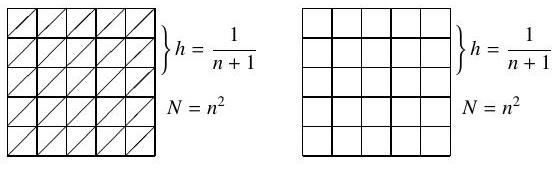
\includegraphics[max width=\textwidth]{2022_01_06_c2f144dbff0f0a17cc7dg-5}

Fig. 1.1. Two-dimensional uniform grid for finite element and finite difference

\subsection{Finite element methods}
We consider two finite elements: continuous linear element and bilinear element. These two finite element methods find $u_{h} \in V_{h}$ such that
$$
\left(\nabla u_{h}, \nabla v_{h}\right)=\left(f, v_{h}\right), \forall v_{h} \in V_{h} .
$$
The above formulation can be written as
$$
\underline{A u}=\underline{f}
$$
with $\underline{A}_{(j-1) n+i,(l-1) n+k}=\left(\nabla \phi_{k l}, \nabla \phi_{i j}\right), f_{(j-1) n+i,(l-1) n+k}=\left(f, \phi_{i j}\right) .$

Basis functions $\phi_{i j}$ satisfy
$$
\phi_{i j}\left(x_{k}, y_{l}\right)=\delta_{(i, j),(k, l)}
$$

\subsubsection{Linear finite element}
Continuous linear finite element discretization of (1.11) on the left triangulation in Fig 1.2. The discrete space for linear finite element is
$$
\mathcal{V}_{h}=\left\{v_{h}:\left.v_{h}\right|_{K} \in P_{1}(K) \text { and } v_{h} \text { is globally continuous }\right\}
$$
Denote $E_{i, j}=\left[x_{i}, x_{i+1}\right] \times\left[y_{i}, y_{i+1}\right]=K_{i, j}^{U} \cup K_{i, j}^{D} .$ For linear element case,

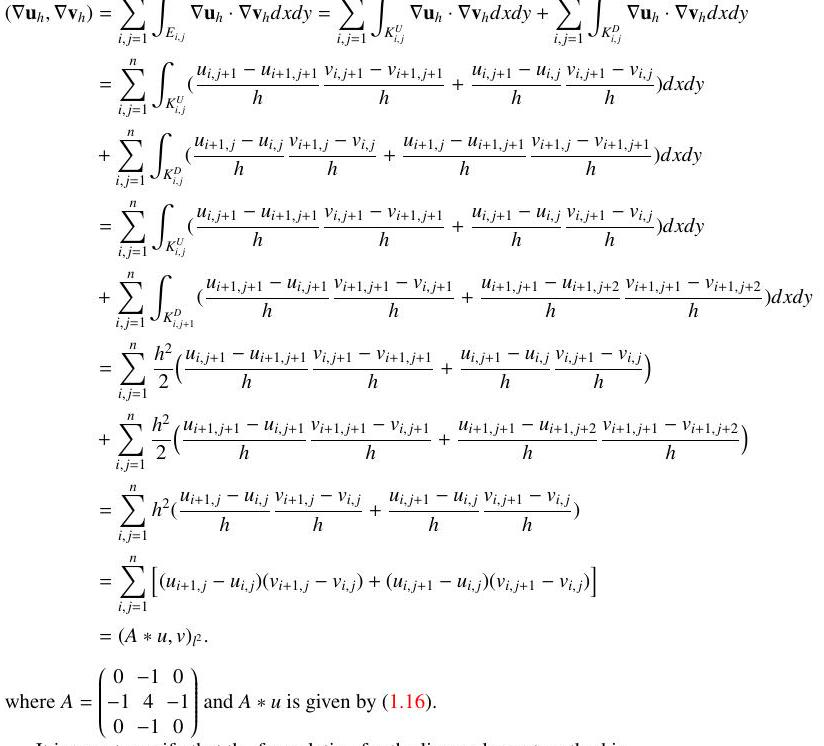
\includegraphics[max width=\textwidth]{2022_01_06_c2f144dbff0f0a17cc7dg-6}

It is easy to verify that the formulation for the linear element method is

(1.16) $4 u_{i, j}-\left(u_{i+1, j}+u_{i-1, j}+u_{i, j+1}+u_{i, j-1}\right)=f_{i, j}, \quad u_{i, j}=0$ if $i$ or $j \in\{0, n+1\}$,

where
$$
f_{i, j}=\int_{\Omega} f(x, y) \phi_{i, j}(x, y) \mathrm{d} x \mathrm{~d} y \approx h^{2} f\left(x_{i}, y_{j}\right)
$$
Proposition 1. The mapping A* has following properties

    \begin{enumerate}
      \item A is symmetric, namely
    \end{enumerate}
$$
(A * u, v)_{l^{2}}=(u, A * v)_{l^{2}} .
$$

    \begin{enumerate}
      \setcounter{enumiii}{2}
      \item $(A * v, v)_{F}>0$, if $v \neq 0$.

      \item $A * u=f$ if and only if

    \end{enumerate}
$$
u \in \underset{v \in \mathcal{V}_{h}}{\arg \min } J(v)=\frac{1}{2}(A * v, v)-(f, v)
$$

    \begin{enumerate}
      \setcounter{enumiii}{4}
      \item The eigenvalues $\lambda_{k l}$ and eigenvectors $u^{k l}$ of A are given by
    \end{enumerate}
$$
\begin{gathered}
\lambda_{k l}=4\left(\sin ^{2} \frac{k \pi}{2(n+1)}+\sin ^{2} \frac{l \pi}{2(n+1)}\right), \\
u_{i j}^{k l}=\sin \frac{k i \pi}{n+1} \sin \frac{l j \pi}{n+1}, 1 \leq i \leq n, 1 \leq j \leq n,
\end{gathered}
$$
and $\rho(A)<8 .$ Furthermore,
$$
\lambda_{n, n}=8 \cos ^{2} \frac{\pi}{2(n+1)} \approx 8\left(1-\left(\frac{\pi}{2(n+1)}\right)^{2}\right) \approx 8-\frac{2 \pi^{2}}{(n+1)^{2}}
$$

\subsubsection{Bilinear element}
Continuous bilinear finite element discretization of (1.11) on the right mesh in Fig. 1.2. The discrete space for linear finite element is
$$
\mathcal{V}_{h}=\left\{v_{h}:\left.v_{h}\right|_{K} \in\{1, x, y, x y\} \text { and } v_{h} \text { is globally continuous }\right\}
$$
For bilinear element case, we have
$$
\begin{aligned}
\left(\nabla \mathbf{u}_{h}, \nabla \mathbf{v}_{h}\right)=& \sum_{i, j=1}^{n} \int_{E_{i, j}} \nabla \mathbf{u}_{h}, \nabla \mathbf{v}_{h} d x d y \\
=& \sum_{i, j=1}^{n} \int_{E_{i, j}}\left(\frac{\left(u_{i+1, j}-u_{i, j}\right)\left(y_{j+1}-y\right)}{h^{2}}+\frac{\left(u_{i, j+1}-u_{i+1, j+1}\right)\left(y-y_{j}\right)}{h^{2}}\right) \\
&\left(\frac{\left(v_{i+1, j}-v_{i, j}\right)\left(y_{j+1}-y\right)}{h^{2}}+\frac{\left(v_{i, j+1}-v_{i+1, j+1}\right)\left(y-y_{j}\right)}{h^{2}}\right) \\
&+\left(\frac{\left(u_{i, j+1}-u_{i, j}\right)\left(x_{i+1}-x\right)}{h^{2}}+\frac{\left(u_{i+1, j}-u_{i+1, j+1}\right)\left(x-x_{i}\right)}{h^{2}}\right) \\
=&\left(\frac{\left(v_{i, j+1}-v_{i, j}\right)\left(x_{i+1}-x\right)}{h^{2}}+\frac{\left(v_{i+1, j}-v_{i+1, j+1}\right)\left(x-x_{i}\right)}{h^{2}}\right) d x d y
\end{aligned}
$$
where $A=\left(\begin{array}{ccc}-1 & -1 & -1 \\ -1 & 8 & -1 \\ -1 & -1 & -1\end{array}\right)$ and $A * u$ is given by $(1.20)$

And we have

(1.20) $8 u_{i j}-\left(u_{i+1, j}+u_{i-1, j}+u_{i, j+1}+u_{i, j-1}+u_{i+1, j+1}+u_{i-1, j-1}+u_{i-1, j+1}+u_{i+1, j-1}\right)=f_{i, j}$, and $u_{i, j}=0$ if $i$ or $j \in\{0, n+1\} .$ References


\end{document}